\documentclass{zc-ust-hw}

\usepackage{lipsum}

\name{SalahDin Ahmed Salh Rezk}
\id{202201079}
\course{COURSE (CODE)}
\assignment{Assignment \#}

\begin{document}

\maketitle

\begin{enumerate}

  %%%%%%%%%%%%%%%%%%%%
  \item Question Number 1
    %%%%%%%%%%%%%%%%%%%%

    \[
      f(x) = x^4 - 2x + 1
    .\] 
    \begin{sol}
      \begin{align}
        F(x) = \int_{0}^{x} f(t) \, dt
      .\end{align}
    \end{sol}

    %%%%%%%%%%%%%%%%%%%%
  \item Question Number 2
    %%%%%%%%%%%%%%%%%%%%

    \begin{figure}[H]
      \centering
      \begin{minipage}{0.7\textwidth}
\begin{lstlisting}[language=Python]
import numpy as np
import matplotlib.pyplot as plt

def f(x):
"""Function to integrate."""
return x**4 - 2*x + 1

def integral(x):
"""Analytical solution of the integral of f(x)."""
return (1/5)*x**5 - x**2 + x

# Plotting
fig, ax = plt.subplots()
x = np.linspace(0, 2, 100)
ax.plot(x, f(x), label='f(x)')
ax.plot(x, integral(x), label='F(x)')
plt.show()
      \end{lstlisting}
    \end{minipage}
    \hfill
    \begin{subfigure}{0.25\textwidth}
      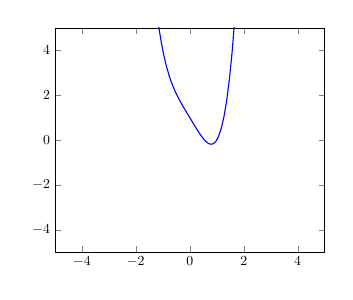
\begin{tikzpicture}[scale=0.5]
        \begin{axis}[
          xmin=-5, xmax=5,
          ymin=-5, ymax=5,
          ]
          \addplot[domain=-5:5, samples=100, color=blue, thick]{x^4-2*x+1};
        \end{axis}
      \end{tikzpicture}
      \caption{$f(x) = x^4 - 2x + 1$}
      \vspace{1em}
      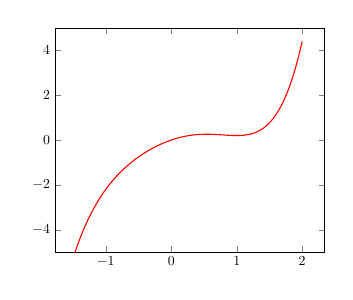
\begin{tikzpicture}[scale=0.5]
        \begin{axis}[
          ymin=-5, ymax=5,
          ]
          \addplot[domain=-2:2, samples=100, color=red, thick]{(1/5)*x^5-x^2+x};
        \end{axis}
      \end{tikzpicture}
      \caption{$F(x) = \frac{1}{5}x^5 - x^2 + x$}
    \end{subfigure}
  \end{figure}

  %%%%%%%%%%%%%%%%%%%%
\item Question Number 3
  %%%%%%%%%%%%%%%%%%%%

  \lipsum[1][1-3]

  \begin{figure}[H]
    \begin{center}
      \begin{circuitikz}[scale=0.95]
        \draw (0,0) to [short, *-] (6,0)
          to [V, l=$V_s$] (6,3)
          to [R, l=$R_1$] (3,3)
          to [R, l=$R_2$] (0,3)
          to [short, -*] (0,0);
        \draw (3,3) to [R, l=$R_3$] (3,0);
      \end{circuitikz}
    \end{center}
    \caption{}%
    \label{fig:}
  \end{figure}
  

\end{enumerate}

\end{document}
